\chapter{基础功能}
在面试和笔试中,经常会出现这类题目,把C++, Java标准库中的一些函数单独拿出来,让你重新实现。这类题目短小精悍,很能考验一个人的基本功是否扎实。

\section{下一个排列} %%%%%%%%%%%%%%%%%%%%%%%%%%%%%%
\label{sec:nextpermutation}

\subsubsection{描述}
实现C++ STL 中的 \fn{next_permutation()},函数原型如下:

\begin{Code}
/**
 * @brief 返回下一个排列,例如当前排列是12345,下一个是12354
 * @param[inout] num 当前排列,例如 12345
 * @param[in] len num的长度
 * @return 无
 */
void next_permutation(int num[], int len);
\end{Code}

\subsubsection{分析}
算法过程如图~\ref{fig:permutation}所示(来自\myurl{http://fisherlei.blogspot.com/2012/12/leetcode-next-permutation.html})。

\begin{center}
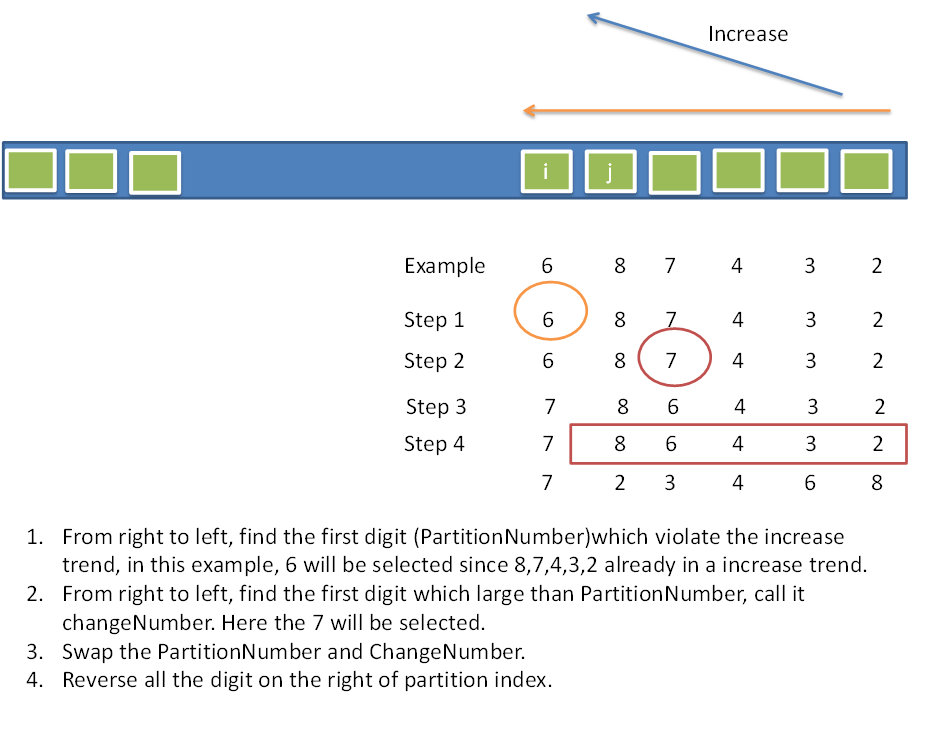
\includegraphics[width=360pt]{next-permutation.png}\\
\figcaption{下一个排列算法流程}\label{fig:permutation}
\end{center}

\subsubsection{代码}

\begin{Codex}[label=next_permutation.c]
static void swap(int array[], int i, int j) {
    const int tmp = array[i];
    array[i] = array[j];
    array[j] = tmp;
}

static void reverse(int array[], int first, int last) { //左闭右开区间
    last--;
    while (first < last)
        swap(array, first++, last--);
}

/**
 * @brief 返回下一个排列,例如当前排列是12345,下一个是12354
 * @param[inout] num 当前排列,例如 12345
 * @param[in] first 开始位置
 * @param[in] last 结束位置,左闭右开区间
 * @return 成功返回 0,失败返回 -1
 */
int next_permutation(int num[], int first, int last) {
    int i, j;

    i = last - 2;  // partition number's index
    while (i >= 0 && num[i] >= num[i + 1])
        i--;

    if (i == -1) {
        reverse(num, first, last);
        return -1;
    }

    j = last - 1;  // change number's index
    while (num[j] <= num[i])
        --j;
    swap(num, i, j);
    reverse(num, i + 1, last);

    return 0;
}
\end{Codex}

\subsubsection{相关的题目}
与本题相同的题目:
\begindot
\item LeetCode -  Next Permutation, \myurl{http://leetcode.com/onlinejudge\#question_31}
\myenddot


\section{数组循环右移} %%%%%%%%%%%%%%%%%%%%%%%%%%%%%%

\subsubsection{描述}
将一个长度为n的数组A的元素循环右移(ROR, Rotate Right)k位,比如数组 {1, 2, 3, 4, 5}循环右移3位之后就变成{3, 4, 5, 1, 2}。

\subsubsection{方法一}
最直接的做法是另开一个大小一样的数组B,遍历一下,令$B[(i + k) \% n] = A[i]$,再将B的内容写回到A即可。这个方法的时间复杂度为O(n),空间复杂度也为O(n)。代码如下:

\begin{Codex}[label=ror.c]
void ror1(int array[], int n, int k) {
    int i;
    int *B = (int*) malloc(n * sizeof(int));

    k %= n;
    if (k == 0)
        return;

    for (i = 0; i < n; i++) {
        B[(i + k) % n] = array[i];
    }
    for (i = 0; i < n; i++) {
        array[i] = B[i];
    }
}
\end{Codex}

\subsubsection{方法二}
另一种简单的做法,每次将数组中的所有元素右移一位,循环k次。这个方法的时间复杂度为O(n*k),空间复杂度为O(1)。代码如下:

\begin{Codex}[label=ror.c]
void ror2(int array[], int n, int k) {
    int i, tmp;
    k %= n;
    if (k == 0)
        return;

    while (k--) {
        tmp = array[n - 1];
        for (i = n - 1; i > 0; i--) {
            array[i] = array[i - 1];
        }
        array[0] = tmp;
    }
}
\end{Codex}

\subsubsection{方法三}
先将A的元素倒置,即{1, 2, 3, 4, 5}变成{5, 4, 3, 2, 1},然后将前k位倒置,即{3, 4, 5, 2, 1},再将后n-k位倒置,即{3, 4, 5, 1, 2},完成。

证明:记A的前n-k位为X,后k位为Y,则A=XY,将A循环右移k位后,应该得到YX。根据该算法,先将A整体倒置,得到$(XY)^T=Y^TX^T$,然后将前k位倒置,得到$YX^T$,最后将后n-k位倒置,得到YX,正好是所求的结果,证毕。

这个方法的时间复杂度为O(2n),空间复杂度为O(1)。代码如下:

\begin{Codex}[label=ror.c]
static void swap(int array[], int i, int j) {
    const int temp = array[i];
    array[i] = array[j];
    array[j] = temp;
}

static void reverse(int array[], int begin, int end) { //左闭右开区间
    end--;
    while (begin < end)
        swap(array, begin++, end--);
}

void ror3(int *array, int n, int k) {
    k %= n;
    if (k == 0)
        return;

    reverse(array, 0, n);
    reverse(array, 0, k);
    reverse(array, k, n - k);
}
\end{Codex}

这种方法需要对每个位置写入2次,看上去也不怎么好,那有没有更好的呢?

\subsubsection{方法四}
我们要做的只是把每个元素放到它应该在的位置,比如开头的例子,1应该放在4的位置,把1放好之后,4就没地方了,那4应该在哪呢,在2的位置,依此类推,就可以把所有的元素都放好,而且只放了一次。看上去这样做很完美,但仔细想想就能想出反例子,比如{1, 2, 3, 4, 5, 6, 7, 8, 9}右移3位,就是1放在4个位置,4放在7的位置,然后7放回1,这时候一圈兜完了,但只排好了3个元素,剩下的6个元素没有动过,怎么办呢?继续下一个,就是2,然后2、5、8也排好了,继续3、6、9,这时候下一个元素是1了,应该停止了(因为1、4、7已经排好了),那程序怎么会知道停在这里了,于是就想到了最大公约数,9和3的最大公约数是3,于是做前3个数的循环就可以了,为什么上一个例子只需做一次,因为元素个数(5)和移动位数(3)互质。具体的数学证明略。

代码如下:

\begin{Codex}[label=ror.c]
static int gcd(int a, int b) {
    assert(a >= b);
    if (b == 0) {
        return a;
    }

    while (b > 0) {
        int tmp = a % b;
        a = b;
        b = tmp;
    }

    return a;
}

void ror4(int *array, int n, int k) {
    int i;
    const int g = gcd(n, k);

    k %= n;
    if (k == 0)
        return;

    for (i = 0; i < g; ++i) {
        int j = i;
        int cur = array[j], tmp;

        do {
            tmp = array[(j + k) % n];
            array[(j + k) % n] = cur;
            cur = tmp;
            j = (j + k) % n;
        } while (j != i);
    }
}

// test
int main(void) {
    int i;
    int a[] = { 1, 2, 3, 4, 5 };
    ror4(a, 5, 3);
    for (i = 0; i < 5; i++) {
        printf("%d ", a[i]);
    }

    return EXIT_SUCCESS;
}
\end{Codex}
